%---------- Inleiding ---------------------------------------------------------

% TODO: Is dit voorstel gebaseerd op een paper van Research Methods die je
% vorig jaar hebt ingediend? Heb je daarbij eventueel samengewerkt met een
% andere student?
% Zo ja, haal dan de tekst hieronder uit commentaar en pas aan.

%\paragraph{Opmerking}
%Dit voorstel is gebaseerd op het onderzoeksvoorstel dat werd geschreven in het
%kader van het vak Research Methods dat ik (vorig/dit) academiejaar heb
%uitgewerkt (met medestudent Mohammed-Ali Kasraoui als mede-auteur).
 
\section{Inleiding}%
\label{sec:inleiding}

% Waarover zal je bachelorproef gaan? Introduceer het thema en zorg dat volgende zaken zeker duidelijk aanwezig zijn:

%\begin{itemize}
%  \item kaderen thema
%  \item de doelgroep
%  \item de probleemstelling en (centrale) onderzoeksvraag
%  \item de onderzoeksdoelstelling
% \end{itemize}
%
%Denk er aan: een typische bachelorproef is \textit{toegepast onderzoek}, wat betekent dat je start vanuit een concrete probleemsituatie in bedrijfscontext, een \textbf{casus}. Het is belangrijk om je onderwerp goed af te bakenen: je gaat voor die \textit{ene specifieke probleemsituatie} op zoek naar een goede oplossing, op basis van de huidige kennis in het vakgebied.

%De doelgroep moet ook concreet en duidelijk zijn, dus geen algemene of vaag gedefinieerde groepen zoals \emph{bedrijven}, \emph{developers}, \emph{Vlamingen}, enz. Je richt je in elk geval op it-professionals, een bachelorproef is geen populariserende tekst. Eén specifiek bedrijf (die te maken hebben met een concrete probleemsituatie) is dus beter dan \emph{bedrijven} in het algemeen.

%Formuleer duidelijk de onderzoeksvraag! De begeleiders lezen nog steeds te veel voorstellen waarin we geen onderzoeksvraag terugvinden.

%Schrijf ook iets over de doelstelling. Wat zie je als het concrete eindresultaat van je onderzoek, naast de uitgeschreven scriptie? Is het een proof-of-concept, een rapport met aanbevelingen, \ldots Met welk eindresultaat kan je je bachelorproef als een succes beschouwen?

%-------------------------------------------------------Inleiding-------------------------------------------------

In veel publieke en private dienstverlenende omgevingen, zoals ziekenhuizen en overheidskantoren is er onvoldoende inzicht in de bezettingsgraad en wachttijden. Methoden voor het menen hiervan zijn vaak onnauwkeurig of niet real-time wat kan leiden tot frustraties en inefficiënt gebruik van middelen. Voor dit probleem is er een duidelijke behoefte aan een geautomatiseerd real-time systeem die zowel de huidige situatie als toekomstige drukte kan voorspellen. Hoewel IoT-technologie veelbelovend is, is het nog niet duidelijk hoe effectief deze oplossing is in de praktijk.

\subsubsection*{Probleemstelling}
In veel publieke en private dienstverlenende omgevingen, zoals ziekenhuizen, overheidskantoren, zijn wachtruimtes vaak drukbezet zonder inzicht in de bezettingsgraad of wachttijden. Dit maakt het efficiënt beheer van de bezoekersstromen en personeelsinzet moeilijker. Traditionele meetmethodes zijn vaak handmatig, onnauwkeurig of niet real-time, dit kan leiden tot frustratie bij bezoekers en suboptimaal gebruik van middelen. Er is dus een duidelijke nood aan geautomatiseerde systemen die real-time inzicht kunnen bieden in deze dynamiek en toekomstige drukte voorspellen. Hoewel IoT-sensoren beschikbaar zijn, is het nog onvoldoende duidelijk hoe praktisch toepasbaar ze zijn in wachtruimtes. Tijdens een gesprek met een medewerker in een dienstverlenende omgeving bleek dat een gebrek aan inzicht in bezettingsgraad en  wachttijden een reëel probleem vormt, wat de relevantie van dit onderzoek benadrukt.


\subsubsection*{Doel van het onderzoek}
Dit onderzoek onderzoekt IoT-technologieën een daadwerkelijke oplossing kan zijn om wachtruimtebezetting in real-time in kaart te brengen, transparant te maken en beter te voorspellen, als ondersteuning voor efficiënter bezoekersbeheer. De focus ligt op het valideren van de werking van het meetsysteem en het verzamelen van basisdata voor voorspellende analyses, niet op het onmiddellijk verkorten van wachttijden.


\subsubsection*{Onderzoeksvraag}
De centrale onderzoeksvraag in dit onderzoek luidt: "Hoe kan IoT-technologie worden ingezet om de bezettingsgraad van wachtruimtes in real-time te meten en voorspellende analyses toe te passen, met als doel het inzicht in bezettingsgraden te verbeteren en zo een basis te bieden voor efficiënter bezoekersbeheer." Om deze vraag te beantwoorden, is het belangrijk om een antwoord te geven op een aantal deelvragen in het probleem- en oplossingsdomein. 

Probleem domein:
\begin{itemize}
    \item Welke beperkingen ondervinden dienstverlening instellingen momenteel bij het meten van bezettingsgraden in wachtruimtes?
    \item Waarom is het verkrijgen van accurate en real-time bezettingsdata essentieel voor het optimaliseren van bezoekersstromen?
    \item Welke uitdagingen zijn er bij het handmatig meten en analyseren van wachttijden?
    \item Wat zijn de eisen waaraan een meetsysteem moet voldoen om als betrouwbaar alternatief te dienen?
\end{itemize}

Oplossing domein:
\begin{itemize}
    \item Welke criteria worden gebruikt om sensoren met elkaar te vergelijken in het kader van een Proof-of-Concept en hoe worden deze criteria gebruikt om IoT-oplossingen te evalueren ten opzichte van bestaande systemen zoals Google Occupancy Analytics?
    \item Hoe kan Little’s Law toegepast worden op de verzamelde IoT-gegevens om inzicht te krijgen in wachttijden?
    %\item Hoe kan een timeseries database effectief worden gebruikt voor het opslaan en analyseren van bezettingsdata?
    \item Op welke manier draagt voorspellende data-analyse bij aan het optimaliseren van bezoekers- en personeelsbeheer?
    \item Hoe kan de integratie van sensoren met bestaande infrastructuren efficiënt worden gerealiseerd?
\end{itemize}

\subsubsection*{Onderzoeksdoelstelling}
Dit onderzoek heeft als doel te bepalen hoe IoT-technologie kan worden ingezet om de bezettingsgraad van wachtruimtes real-time te meten en wachttijden te voorspellen. Via de Proof-of-Concept (PoC) wordt nagegaan hoe IoT-sensoren en data-analyse de bezettingsgraad en bezoekersstromen accuraat en privacyvriendelijk in kaart kunnen brengen.

\subsubsection*{Verwachte eindresultaat} 
Het verwachte eindresultaat is een werkende proof-of-concept die aantoont hoe IoT-oplossingen de bezettingsgraad en wachttijden kunnen meten en inzichtelijk maken. Op basis van de resultaten worden aanbevelingen geformuleerd voor mogelijke implementaties.


%---------- Stand van zaken ---------------------------------------------------

\section{Literatuurstudie}%
\label{sec:literatuurstudie}

%Hier beschrijf je de \emph{state-of-the-art} rondom je gekozen onderzoeksdomein, d.w.z.\ een inleidende, doorlopende tekst over het onderzoeksdomein van je bachelorproef. Je steunt daarbij heel sterk op de professionele \emph{vakliteratuur}, en niet zozeer op populariserende teksten voor een breed publiek. Wat is de huidige stand van zaken in dit domein, en wat zijn nog eventuele open vragen (die misschien de aanleiding waren tot je onderzoeksvraag!)?

%Je mag de titel van deze sectie ook aanpassen (literatuurstudie, stand van zaken, enz.). Zijn er al gelijkaardige onderzoeken gevoerd? Wat concluderen ze? Wat is het verschil met jouw onderzoek?

% Verwijs bij elke introductie van een term of bewering over het domein naar de vakliteratuur, bijvoorbeeld~\autocite{Hykes2013}! Denk zeker goed na welke werken je refereert en waarom.

%Draag zorg voor correcte literatuurverwijzingen! Een bronvermelding hoort thuis \emph{binnen} de zin waar je je op die bron baseert, dus niet er buiten! Maak meteen een verwijzing als je gebruik maakt van een bron. Doe dit dus \emph{niet} aan het einde van een lange paragraaf. Baseer nooit teveel aansluitende tekst op eenzelfde bron.

%Als je informatie over bronnen verzamelt in JabRef, zorg er dan voor dat alle nodige info aanwezig is om de bron terug te vinden (zoals uitvoerig besproken in de lessen Research Methods).

% Voor literatuurverwijzingen zijn er twee belangrijke commando's:
% \autocite{KEY} => (Auteur, jaartal) Gebruik dit als de naam van de auteur
%   geen onderdeel is van de zin.
% \textcite{KEY} => Auteur (jaartal)  Gebruik dit als de auteursnaam wel een
%   functie heeft in de zin (bv. ``Uit onderzoek door Doll & Hill (1954) bleek
%   ...'')

%Je mag deze sectie nog verder onderverdelen in subsecties als dit de structuur van de tekst kan verduidelijken.


\subsection{Inleiding}
Het internet of Things (IoT) is een snel evoluerende technologie met toepassingen allerlei gebieden zoals industrie, mobiliteit en slimme steden. Miljarden verbonden apparaten verzamelen continu gegevens wat automatisering en betere geïnformeerde besluitvorming mogelijk maakt. Dit leidt tot efficiëntere processen en optimaler gebruik van middelen. Een gebied waar IoT nuttig kan zijn, is in wachttijdsgerelateerde problemen. Die ontstaan vaak omdat vraag en aanbod niet goed op elkaar afgestemd zijn. In sectoren zoals publieke diensten, logistiek en klantendiensten  kan dit leiden tot inefficiëntie of zelfs ernstige maatschappelijke gevolgen.

\subsection{Overzicht Internet of Things}
De term Internet of Things (IoT) ontstond in 1999, toen de Britse technologiepionier Kevin Ashton objecten via RFID-tags met het internet wilde verbinden \autocite{Bassi2013, Rejeb2023}. IoT verwijst naar een netwerk van fysieke objecten die, uitgerust met sensoren en actuatoren, gegevens verzamelen, verwerken en uitwisselen, waardoor ze slim en interactief worden \autocite{Elksasy2023}. Het concept wordt gezien als een manier waarop objecten continu met elkaar verbonden zijn, onafhankelijk van plaats, tijd, medium of netwerk (zie Figuur \ref{fig:Figuur9}).

\begin{figure}[h]
  \centering
  \includegraSource: \autocite{Dauwed2018}}
\end{figure}phics[width=0.4\textwidth]{img/iot-concept.jpg}
  \caption{Internet of Things Networking}
  \label{fig:Figuur9}
  \textit{

\subsection{IoT hardware componenten} 
Een IoT-omgeving bestaat uit verschillende kerncomponenten zoals sensoren, actuatoren, microprocessors, en communicatie protocollen. Deze maken het mogelijk dat apparaten slim worden en met elkaar te communiceren \autocite{Abraham2023, Gharde2024}. In de volgende secties worden deze componenten verder behandeld om inzicht te geven in de werking van IoT. De eerste component dat geanalyseerd zal worden zijn de sensoren.

\subsubsection{Sensors}
Sensoren vormen een essentieel onderdeel van een IoT-systeem en worden gebruikt om  chemische veranderingen en anomalieën te detecteren \autocite{Abraham2023, Moyer2019, Sehrawat2019}. Het IoT-systeem wordt compleet wanneer deze gegevens gecombineerd worden met actuatoren, die in het volgende sectie worden besproken. 

\subsection*{Sensor types en het gebruik ervan} \autocite{Moyer2019, Sehrawat2019, Kumar2024, Balogun2017, Meenakshi2020, Tresanchez2018, Shanmugavalli2023, Gala2020, Gade2013, Chidurala2021, Karunarathne2018, Srinivasan2022}

\begin{enumerate}
    \item \textbf{Motion sensor:} Een bewegingsdetector is een IoT-apparaat dat fysieke beweging detecteert en ingezet worden voor het detecteren van een inbraak. Zo gebruiken \autocite{Tiong2019} motion sensing in een IoT-gebaseerd beveiligingssysteem voor thuis.
   
    \item \textbf{Pressure sensor:} Een druksensor in IoT-systemen meet en detecteert kracht en drukte en wordt gebruikt om de bezetting van stoelen en bedden real-time te monitoren.
    
    \item \textbf{Optical proximity sensor:} Wordt gebruikt voor het detecteren van objecten door gebruik te maken van licht zonder fysiek contact.
    
    \item \textbf{Wireless Communication:} Is een belangrijk aspect van IoT. Deze zorgt ervoor dat devices met elkaar kunnen communiceren door data te delen en verzenden.
    
    \item \textbf{Thermal camera:} Thermische camera's detecteren infrarode radiatie van objecten met een temperatuur hoger dan nul graden en kunnen worden ingezet voor het monitoren van niet-intrusieve bezetting.
    
    \item \textbf{Proximity sensors:} Proximity sensoren, meestal gebruikt in de in de industrie en landbouw, detecteren nabijheid van objecten via elektromagnetische velden.
    
    \item \textbf{Image sensors:} Beeldsensoren gebruiken fotodiodes om licht in een bepaald gebied te detecteren. Deze worden toegepast in medische beeldvorming, digitale camera's, nachtzichtapparatuur  en klantmonitoring in winkels

\end{enumerate}

\begin{enumerate}
    \item \textbf{Motion sensor}
    \begin{enumerate}
        \item \textbf{Passive Infrared (PIR) sensors:} Detecteert beweging door veranderingen te waarnemen in infraroodstraling.
        \item \textbf{Microwave:} Deze sensor zendt microgolven uit, de reflectie van deze golven wordt geanalyseerd om beweging te detecteren.
        \item \textbf{Ultrasonic:} Zendt en ontvangt geluidsgolven boven de 20 kHz om beweging te detecteren, samen met de afstand tussen objecten.
    \end{enumerate}
    
   % \item \textbf{Pressure sensor}
   % \begin{enumerate}
   %     \item \textbf{Force-Sensitive Resistors:} Is een low-cost pressure sensor waarbij de weerstand verandert wanneer kracht gedetecteerd wordt.
   %     \item \textbf{Strain Gauge Pressure Sensors:} Meet drukte door de deformatie van een materiaal te detecteren.
   % \end{enumerate}
    
    \item \textbf{Optical proximity sensors}
    \begin{enumerate}
        \item \textbf{Infrared break beam sensor:} Een infrarood emitter en een receiver worden tegenover elkaar geplaatst waardoor er een infrarood licht ontstaat. Wanneer een persoon door het licht gaat, wordt deze onderbroken waardoor er een detectie geactiveerd wordt.
        \item \textbf{Diffuse Reflective Optical Sensor:} \\ Wordt gebruikt voor objectdetectie en nabijdetectie. Deze sensoren zenden licht uit en meten het gereflecteerde licht van objecten waardoor ze deze kunnen detecteren.
    \end{enumerate}
    
    \item \textbf{Wireless communication protocol}
    \begin{enumerate}
        \item \textbf{BLE (Bluetooth Low Energy) beacon:} Zijn wireless zenders die unieke identifiers uitzenden.
        \item \textbf{Radio Frequency Identification (RFID):} Bestaat uit een tag, reader en middleware software. Maakt gebruik van radiogolven om data draadloos te verzenden.
    \end{enumerate}
    
   % \item \textbf{Thermal camera}
   %  \begin{enumerate}
   %      \item \textbf{Uncooled thermal camera:} Een device voor het detecteren van infraroodradiatie zonder de nood voor een koelsysteem.
   %      \item \textbf{Cooled thermal camera:} Detecteert infrarode radiatie met hoge snelheid en gevoeligheid door de sensoren naar cryogenische temperaturen te laten dalen.
   %  \end{enumerate}
    
    \item \textbf{Proximity sensors}
    \begin{enumerate}
        \item \textbf{Inductief:} Detecteert geleidende en niet-geleidende materialen door middel van een elektromagnetisch veld.
        \item \textbf{Capacitief:} Maakt gebruik van zwakke elektrische velden om geleidende en niet-geleidende materialen te detecteren.
        \item \textbf{Ultrasoon:} Wordt gebruikt om nabijheid en afstand te meten door middel van een hoogfrequente geluidsgolf.
    \end{enumerate}
    
    \item \textbf{Image sensors}
    \begin{enumerate}
        \item \textbf{Linear image sensor:} Legt lijn voor lijn afbeeldingen vast waardoor real-time tracking van stoelbezetting mogelijk is. Kan in de gezondheidszorg gebruikt worden om de bezetting van wachtruimtes en patiëntenflow te monitoren.
        \item \textbf{Infrared Image Sensors:} Detecteert infraroodradiatie en converteert het naar een beeld.
    \end{enumerate}
\end{enumerate}


\subsubsection{Actuatoren}
Actuatoren zijn componenten die in staat zijn om het “fysieke wereld” te beïnvloeden op basis van de verzamelde gegevens \autocite{Moyer2019}. Actuatoren werken in samenwerking met sensoren om een compleet IoT-systeem te creëren. In de volgende sectie wordt het IoT-systeem verder toegelicht door de rol van de microprocessoren te introduceren.

\subsubsection{Microprocessors}
Microprocessoren spelen een essentiële rol in IoT-systemen. Deze fungeren als de centrale eenheid in een IoT-device en zijn verantwoordelijk voor het verwerken van sensorgegevens, uitvoeren van berekeningen en het besturen van actuatoren \autocite{Abraham2023, James2021}. In de volgende sectie worden de communicatieprotocollen besproken, die een essentiële onderdeel vormen van IoT-systemen.

\subsubsection{Communicatie protocollen}
Communicatieprotocollen faciliteren de communicatie tussen twee slimme apparaten. Wat betreft IoT werden er diverse communicatieprotocollen ontwikkeld zoals HTTP, MQTT en XMPP. De keuze hangt af van factoren zoals energie-efficiëntie, veiligheid en kwaliteit van de dienstverlening \autocite{Anitha2022, Jeddou2020}. 

\subsection{Implementaties van IoT in wachtruimtes} \label{wachtruimte}

\begin{enumerate}
    \item \textbf{Daniele Spoladore et al. (2024) – Italië}
    \begin{itemize}
        \item \textbf{Doelstelling:} Onderzoeken hoe IoT, AI en Virtual Reality een wachtruimte kunnen transformeren in een smart omgeving.
        \item \textbf{Toepassing van IoT:} De Age-IT prototype maakt gebruik van IoT-sensoren, AI en Virtual Reality. Hoewel de autheurs verwijzen naar IoT-sensoren worden de specifieke types niet vermeld.
        \item \textbf{Conclusie:} Dit systeem biedt een significante stap bij het transformeren van traditionele wachtruimtes in een smart omgeving en het omzetten van wachttijden in diagnostische en therapeutische activiteiten.
    \end{itemize}
    
    \item \textbf{M. Ghazal et al. (2015) – Bahrein}
    \begin{itemize}
        \item \textbf{Doelstelling:} Verbeteren van queue management door de servicekwaliteit te verhogen en wachttijden te verminderen.
        \item \textbf{Toepassing van IoT:} Het systeem maakt gebruik van een ESP32-module om live wachtrijgegevens te versturen.
        \item \textbf{Conclusie:} Het systeem functioneert zoals beschreven in de studie.
    \end{itemize}
\end{enumerate}


\subsection{Bezettingsdetectiesystemen: Sensor-gebaseerde vs Vision-gebaseerde IoT-oplossingen}
bezettingsdetectie systemen detecteren of een ruimte bezet of onbezet is, met behulp van verschillende detectiemethoden \autocite{Kleiminger2015}. Deze methoden kunnen grofweg worden gecategoriseerd als IoT- en niet-IoT-systemen \autocite{Chaudhari2024}.

\subsubsection{IoT-based detectiesystemen}
IoT gebaseerde systemen maken gebruik van verschillende sensoren en algoritmes om de aanwezigheid van mensen te detecteren. Omgevingssensoren kunnen de bezetting detecteren door veranderingen in CO2-niveaus en temperatuur, zelfs als de bewoners stilstaan \autocite{Chand2021}. Veelgebruikte technologieën zijn bewegingssensoren, IR-sensoren, ultrasoon sensoren en IoT-omgevingssensoren \autocite{Ji2018, Hammoud2017}.

\subsubsection{Voordelen}
\begin{itemize}
    \item  Nauwkeurigheid: zeer nauwkeurig in het tellen van individuen en het detecteren van aanwezigheid, vooral in gecontroleerde omgevingen \autocite{Chaudhari2024, Khan2024}.
    \item Privacy: biedt een privacybehoudende alternatief voor traditionele, op camera's gebaseerde methoden. \autocite{Yang2018}
\end{itemize}}

\subsubsection{Nadelen}
\begin{itemize}
    \item  Plaatsing van sensoren: sterk afhankelijk van strategische plaatsing van sensoren voor optimale prestaties. Verkeerde plaatsing kan leiden tot onbetrouwbare gegevens en foutieve metingen. \autocite{Chaudhari2024, Begovic2024}
    \item  Beperkte bereik: beperkingen in bereik en nauwkeurigheid, vooral in grote ruimtes \\ \autocite{Chaudhari2024}. 
\end{itemize}

\subsubsection{Vision-gebaseerde IoT-oplossingen: \\ Google Occupancy Analytics Suit}
Google biedt een breed scala aan cloudtools en API’s waarmee ontwikkelaars krachtige applicaties en visualisaties kunnen maken \autocite{Dincer2013}. Een veelgebruikte tool is de Google Occupancy Analytics Suite. Dit is een verzameling van de voorgetrainde AI-modellen van Vertex AI Vision en AutoML-tools die worden gebruikt voor het tellen van mensen of voertuigen op basis van videobeelden. \autocite{Cloud2025, Cloud2025a}.

\subsubsection{Voordelen} \autocite{Cloud2025}
\begin{itemize}
    \item Privacy: Kan worden geïmplementeerd met Person / Face Blur model om privacy te waarborgen
    \item Opslag: Data wordt naar BigQuery verstuurt om gestructureerde gegevens op te slaan in een tabel.
\end{itemize}

\subsubsection{Nadelen} \autocite{Cloud2025}
De volgende factoren kunnen de prestaties van het model verminderen: 
\begin{itemize}
    \item Slechte lichtomstandigheden.
    \item Drukte en occlusie van objecten.
    \item Ongebruikelijke of minder gebruikelijke gezichtspunten.
    \item Kleine objecten.
\end{itemize}

\subsubsection{Vergelijking tussen IoT-oplossingen en Google Occupancy}
Zowel IoT-gebaseerde detectiesystemen als vision-gebaseerde IoT-detectiesystemen oplossingen, zoals Google Occupancy Analytics Suite, bieden mogelijkheden ruimtebezetting te monitoren. IoT-systemen bieden meer privacy omdat ze geen videobeelden gebruiken en functioneren goed bij slechte verlichting maar zijn gevoelig voor plaatsing en hebben beperkt bereik. De Google Occupancy Analytics Suite daarentegen gebruikt videobeelden en AI om personen nauwkeurig te tellen zelfs in complexe situaties. De beeldverwerking gebeurt hierbij niet lokaal, maar volledig in de cloud via de Vertex AI Vision-dienst van Google. Hoewel het systeem gebruikmaakt van blur-algoritmen om gezichten en personen te anonimiseren, blijven er privacyvragen bestaan vanwege de aard van cameragebaseerde monitoring en het gebruik van cloudverwerking.

%\subsection{Timeseries databases}
%In IoT-omgevingen genereren sensoren enorme hoeveelheden tijdsgebaseerde gegevens \autocite{Sgueglia2022, Ramachandran2018}. Time-series databases zijn gespecialiseerde systemen voor het behandelen van grote volumes data die over de tijd veranderd. InfluxDB, OpenTSDB en TimescaleDB zijn onder de meest populaire time-series database management systems (TSDBMSs) \autocite{Zymbler2021}.

\subsection{Little’s Law en wachttijdanalyse}
De wet van Little is een fundamentele principe in wachtrij theorie, dat de relatie toont tussen het gemiddelde aantal items of personen in een systeem \(L\), de gemiddelde aankomstsnelheid (\( \lambda \)) en de gemiddelde tijd doorbracht in het systeem \(W\). \autocite{Little2008, Wolff2011}

\[
L = \lambda W
\]

\subsubsection{Steady-State Aannames voor Little's Law}
Little's Law gaat uit van een steady-state \autocite{Walsh2007} waarbij de aankomstsnelheid gelijk is aan de vertreksnelheid \autocite{Marks2019}. Dit kan problematisch zijn door fluctuaties in het systeem \autocite{Walsh2007} waardoor het moeilijk is om snelheden nauwkeurig te meten \autocite{Hayati2017}.

\subsubsection{Toepassing van Little’s Law}
De eenvoud en brede toepasbaarheid hebben geleid tot een wijdverspreid gebruik in verschillende gebieden zoals logistiek en dienstverlening \autocite{SimchiLevi2011}. De veelzijdigheid van de wet komt voort uit vier belangrijke factoren: toepasbaarheid, nut, eenvoud en zichtbaarheid. \autocite{Potter2020}

\subsubsection{Relevantie voor dit onderzoek}
In dit project vormt Little’s Law het theoretisch kader om de bezettingsgraad te analyseren. Door gebruik te maken van IoT-technologie worden zowel aankomstsnelheid \( \lambda \) en verblijftijd (\(W\)) gemeten, wat een objectieve berekening van de gemiddelde bezetting (\(L\)) mogelijk maakt. Deze inzichten ondersteunen de evaluatie van de impact van het systeem op de wachttijden. Ook in ziekenhuizen en medische praktijken wordt Little’s Law toegepast om het verband tussen patiënteninstroom, verblijfsduur en bezetting te verklaren \autocite{Aahlin2022}. Hierbij wordt het aantal aanwezige patiënten beschouwd als work-in-process binnen het zorgproces, dit geldt ook voor de wachtzaal in dit onderzoek.

\subsection{Voorbeelden uit de praktijk: bestaande systemen en onderzoeken}
Hieronder worden enkele bestaande systemen en onderzoeken besproken die bezettingsdetectie in de praktijk hebben onderzocht of geïmplementeerd.

\begin{enumerate}
    \item Dit onderzoek stelt een bezettingssysteem voor dat gebruikmaakt van radiogebaseerde frequenties, zoals WiFi en Bluetooth, om de bezetting van een ruimte te detecteren \autocite{Shahbazian2023}.
    
    \item Deze studie onderzoekt en vergelijkt verschillende technologieën voor aanwezigheidsdetectie in gebouwen, met de nadruk op infraroodtechnologieën zoals PIR-sensoren, lichtbarrières en IR-imaging, maar bespreekt ook microgolf- en ultrasoon technologieën. \\ \autocite{Maaspuro2018}
    
    \item Deze studie stelt een deep-learningmodel voor dat op basis van CCTV-beelden zowel het aantal aanwezige personen als hun locaties in gebouwen detecteert. \autocite{Hu2023}
    
    \item De paper onderzoekt hoe een sensornetwerk en machine learning-methodes, zoals Hidden Markov Models, ingezet kunnen worden om bezetting in een open kantoor te schatten op basis van CO₂ en geluid. \autocite{Lam2009}
\end{enumerate}

Op basis van bovenstaande voorbeelden blijkt de combinatie tussen PIR-, ultrasoon- en \\ IR-sensoren een goede balans te bieden tussen nauwkeurigheid, energieverbruik, kostprijs en privacybescherming. Volgens een onderzoek van \autocite{Maaspuro2018}. zijn PIR- en ultrasone sensoren zeer effectief in het detecteren van aanwezigheid in gebouwen omdat ze sterk en energiezuinig zijn. In tegenstelling tot methoden op basis van camerabeelden of WiFi/Bluetooth-signalen \autocite{Hu2023, Shahbazian2023}, \\ biedt de IoT-gebaseerde implementatie een eenvoudiger, minder privacygevoelig alternatief dat geen complexe infrastructuur vereist.


\subsection{Voorspellende modellen op basis van historische data}
Voorspellende modellen worden in verschillende sectoren steeds vaker ingezet om trends in bezoekersaantallen en systeemgebruik te anticiperen \autocite{Ejstrud2006}. Op basis van historische data kunnen algoritmen zoals ARIMA, Random Forest en LSTM-modellen gebruikt worden voor het voorspellen van tijdreeksen, met name om piekmomenten te identificeren \autocite{Park_2024}. 

\subsubsection{Praktische toepassingen}
In een aantal onderzoeken wordt de toepassing van ARIMA-, Random Forest- en LSTM-modellen voor tijdreeksvoorspellingen onderzocht, met name in de context van landbouw en voorraadbeheer \autocite{Nagendra2023}. Deze domeinen tonen het potentieel van dergelijke modellen om processen efficiënter te maken door vooruit te kijken op basis van historische trends.

\subsubsection{Belang van datakwaliteit en granulariteit}
De effectiviteit van deze modellen wordt sterk beïnvloed door de kwaliteit en kwantiteit van de data \autocite{Mani2021}. IoT-technologieën bieden hierbij een voordeel doordat ze real-time en gedetailleerde gegevens kunnen leveren.

\subsubsection{Voordeel van voorspellende modellen}
Recent onderzoek toont aan dat het voorspellen van wachttijden en drukte het middelenbeheer en de klanttevredenheid in verschillende dienstverlenende sectoren aanzienlijk kan verbeteren \autocite{Benevento2021}.



%---------- Methodologie ------------------------------------------------------
\section{Methodologie}%
\label{sec:methodologie}

% Hier beschrijf je hoe je van plan bent het onderzoek te voeren. Welke onderzoekstechniek ga je toepassen om elk van je onderzoeksvragen te beantwoorden? Gebruik je hiervoor literatuurstudie, interviews met belanghebbenden (bv.~voor requirements-analyse), experimenten, simulaties, vergelijkende studie, risico-analyse, PoC, \ldots?

% Valt je onderwerp onder één van de typische soorten bachelorproeven die besproken zijn in de lessen Research Methods (bv.\ vergelijkende studie of risico-analyse)? Zorg er dan ook voor dat we duidelijk de verschillende stappen terug vinden die we verwachten in dit soort onderzoek!

% Vermijd onderzoekstechnieken die geen objectieve, meetbare resultaten kunnen opleveren. Enquêtes, bijvoorbeeld, zijn voor een bachelorproef informatica meestal \textbf{niet geschikt}. De antwoorden zijn eerder meningen dan feiten en in de praktijk blijkt het ook bijzonder moeilijk om voldoende respondenten te vinden. Studenten die een enquête willen voeren, hebben meestal ook geen goede definitie van de populatie, waardoor ook niet kan aangetoond worden dat eventuele resultaten representatief zijn.

%Uit dit onderdeel moet duidelijk naar voor komen dat je bachelorproef ook technisch voldoen\-de diepgang zal bevatten. Het zou niet kloppen als een bachelorproef informatica ook door bv.\ een student marketing zou kunnen uitgevoerd worden.

% Je beschrijft ook al welke tools (hardware, software, diensten, \ldots) je denkt hiervoor te gebruiken of te ontwikkelen.

%Probeer ook een tijdschatting te maken. Hoe lang zal je met elke fase van je onderzoek bezig zijn en wat zijn de concrete \emph{deliverables} in elke fase?

Op basis van de literatuurstudie, waarin verschillende IoT-oplossingen, sensortypes en analysemethoden werden geanalyseerd, worden in dit hoofdstuk de gekozen onderzoeksmethoden toegelicht.


\subsubsection{Devices}
In deze vergelijkende studie worden verschillende types devices met elkaar vergeleken die nodig zijn bij de implementatie van de proof-of-concept. Het identificeren van de devices gebeurt door het raadplegen van de uitgevoerde literatuurstudie en bijkomende onderzoeken. devices worden geïdentificeerd voor de volgende componenten.

\begin{itemize}
    \item Centrale eenheid
    \item Sensor controller
    \item Lichtsluis/IR-sensor
    \item PIR-bewegingssensoren
    \item Ultrasoon/infraroodsensoren
\end{itemize}


\subsubsection{Methodologie van vergelijking}

De vergelijkende studie bevat de volgende criteriums:
\begin{itemize}
    \item \textbf{Centrale eenheid en sensor controller}
    \begin{itemize}
        \item Voor- en nadelen: Een overzicht van de voordelen en nadelen van deze twee componenten.
        \item Kosten: De kostenanalyse omvat enkel de aanschafkosten van deze onderdelen.  
    \end{itemize}
    
\item \textbf{Vergelijking van sensoren}

De volgende sensoren worden met elkaar vergeleken in dit onderzoek: \\
lichtsluis-/infraroodsensoren, \\ PIR-bewegingssensoren, \\ ultrasoon-/infraroodsensoren.

De vergelijking gebeurt op basis van de volgende criteria:

\begin{itemize}
    \item Nauwkeurigheid
    \item Gevoeligheid
    \item Bereik
    \item Connectiviteit
    \item Kostprijs (€)
\end{itemize}
    
    
    %\item \textbf{Betrouwbaarheid:} Hier wordt gekeken naar de stabiliteit van het apparaat, de kwaliteit van de hardware.    
    %\item \textbf{Gebruiksvriendelijkheid:} Dit criterium omvat de eenvoud van installatie, configuratie, bediening.    
    %\item \textbf{Integratie capaciteit:} De mogelijkheid om het IoT apparaat te integreren met andere systemen of apparaten (Raspberry Pi, Arduino) wordt onderzocht. 
\end{itemize}


\section{Procedure: Proof-of-Concept (PoC)}
De Proof-of-Concept (PoC) onderzoekt hoe IoT-technologie kan worden ingezet om wachttijden in kaart te brengen, transparant te maken als basis voor latere optimalisaties. De studie beoogt niet om tijdens de meetperiode effectief een daling van de wachttijd te realiseren.

\subsection{Nulmeting en verzameling van historische gegevens}
Om de effectiviteit van het Proof-of-Concept (PoC) te evalueren, wordt eerst een nulmeting uitgevoerd tijdens een piekmoment. Hierbij wordt gebruikgemaakt van een tool (Google Occupancy Analytics Suite) om de huidige bezettingsgraad van de wachtruimte te meten. Tijdens deze meting worden gegevens verzameld zoals het aantal aanwezigen per tijdseenheid, het verloop van piek- en dalmomenten en indien mogelijk de gemiddelde wachttijden. Deze gegevens vormen de baseline waarmee achteraf de impact van het nieuwe IoT-gebaseerde systeem objectief kan worden beoordeeld. De vergelijking tussen de metingen via Google Occupancy Analytics en het IoT-systeem dient als objectieve validatie van de betrouwbaarheid van het nieuwe meetsysteem. Indien beschikbaar, kunnen ook interne statistieken zoals het aantal afgewerkte dossiers per uur gebruikt worden ter ondersteuning van deze vergelijking.

\subsection{Opbouw van het meetsysteem}
In het Proof of Concept (PoC) wordt een eenvoudige IoT-architectuur gebruikt waarbij sensoren in real-time registreren hoeveel mensen aanwezig zijn. De metingen gebeuren volledig anoniem, zonder tracking op persoonsniveau. De verzamelde gegevens worden automatisch doorgestuurd naar een timeseries database voor opslag. 

\subsection{Technische uitwerking}
Het meetsysteem in deze Proof-of-Concept maakt gebruik van een beperkte selectie sensortechnologieën die anoniem de aanwezigheid van personen in de wachtruimte registreren. Sensoren worden ingezet om de bewegingen van personen binnen de ruimte te detecteren. Aan de ingangen en doorgangen worden sensoren geplaatst voor het nauwkeurig detecteren of iemand een ruimte binnenkomt of verlaat en in welke richting, wat essentieel is om dubbele tellingen te voorkomen. Daarnaast wordt een type sensoren gebruikt om afstanden tot personen te meten. Dit laat toe om ook personen te detecteren, ongeacht of ze staan of zitten, zelfs als zij weinig tot geen beweging vertonen. Door deze sensoren te combineren ontstaat een betrouwbaar beeld van de actuele bezetting, zonder gebruik te maken van camera’s of persoonsgegevens. Alle metingen gebeuren dus volledig privacyvriendelijk en in real-time, waardoor het systeem geschikt is voor toepassing zoals een wachtzaal. 

\subsection{Verbindingen met de Borden}
De sensoren zijn verbonden met de centrale eenheid via de GPIO-pinnen (General Purpose Input/Output). De sensorcontroller fungeert als de centrale controller en stuurt de verzamelde gegevens draadloos naar de centrale eenheid via Wi-Fi, gebruikmakend van een MQTT-protocol of HTTP-API. De centrale eenheid ontvangt deze data en verwerkt ze verder voor opslag in een database. Dit systeem maakt een betrouwbare en efficiënte dataverzameling en -overdracht mogelijk, zonder complexe bedrading.

\subsection{Little's Law-formule}

Little’s Law is een fundamentele formule binnen de wachtrijtheorie en stelt dat:

\[
L = \lambda W
\]

waarbij:
\begin{itemize}
    \item \( L \): het gemiddelde aantal personen in het systeem (bezettingsgraad),
    \item \( \lambda \): de gemiddelde aankomstsnelheid (personen per tijdseenheid),
    \item \( W \): de gemiddelde tijd die een persoon in het systeem doorbrengt.
\end{itemize}

In dit onderzoek wordt Little’s Law gebruikt als theoretisch kader om het belang van bezettingsdata te onderbouwen. De nadruk ligt op het accuraat meten van \( L \) via IoT-sensoren. Aangezien \( \lambda \) en \( W \) binnen de korte meetperiode niet betrouwbaar kunnen worden vastgesteld, wordt er geen exacte berekening van wachttijd uitgevoerd. In plaats daarvan focust de proof-of-concept zich op de validatie van de bezettingsgraad \( L \), als eerste stap naar datagedreven bezoekersanalyse en eventuele latere voorspellingen.


\subsection{Validatie van bezettingsmetingen}
Vooraleer de verzamelde gegevens worden gebruikt voor verdere analyse, wordt gecontroleerd of het meetsysteem correcte en consistente resultaten oplevert. Dit gebeurt via steekproeven waarbij het aantal aanwezigen in de wachtruimte handmatig wordt geteld en vergeleken met de waarden die automatisch door het systeem zijn geregistreerd. Indien afwijkingen worden vastgesteld, wordt het systeem aangepast of opnieuw gekalibreerd. Deze validatie garandeert de betrouwbaarheid van de data voor latere vergelijking met de nulmeting.

\subsection{Verwerking en vergelijking van gegevens}
De resultaten van het IoT-gebaseerde wachttijdbeheersysteem worden vergeleken met de resultaten uit de nulmeting op basis van de bezettingsgraad. Deze vergelijking maakt het mogelijk om objectief te evalueren of het gebruik van IoT-technologie daadwerkelijk leidt tot een vermindering van wachttijden en een efficiënter bezoekersbeheer.

\subsection{Voorspellende analyses}
Op basis van de verzamelde historische gegevens wordt een voorspellend model ontwikkeld. Dit model kan trends en patronen in bezoekersgedrag identificeren, zoals typische piekmomenten per dag of week. Door deze voorspellingen kunnen bezoekers en personeel zich beter voorbereiden op verwachte drukte, wat de wachttijdreductie verder ondersteunt. 

\subsection{Hoe IoT concreet bijdraagt aan wachttijdreductie}
De verzamelde gegevens maken real-time optimalisatie mogelijk doordat het systeem drukke momenten kan voorspellen en zo bijdraagt aan beter personeelsbeheer. Bovendien draagt het systeem bij aan een efficiënter bezoekersbeheer, waardoor de wachttijden beter te voorspellen zijn en bezoekers hun tijd optimaler kunnen benutten.

\subsection{Resultaten}
De resultaten worden als een succes beschouwd wanneer de juiste apparaten zijn geselecteerd, correct zijn geïntegreerd in het systeem, en de verzamelde gegevens consistent en betrouwbaar zijn. Het succes wordt verder bepaald door hoe goed de gegevens van de IoT-sensoren kunnen worden vergeleken met de resultaten van de bestaande tool (Google Occupancy Analytics Suite). Daarnaast moet het systeem aantoonbaar nauwkeurige metingen bieden, die valide zijn bij het vergelijken van de bezettingsgraad en wachttijden.

%\begin{figure}[h]
%    \centering
%    \subsubsection*{Milestone} % Place the subsection above the figure
%    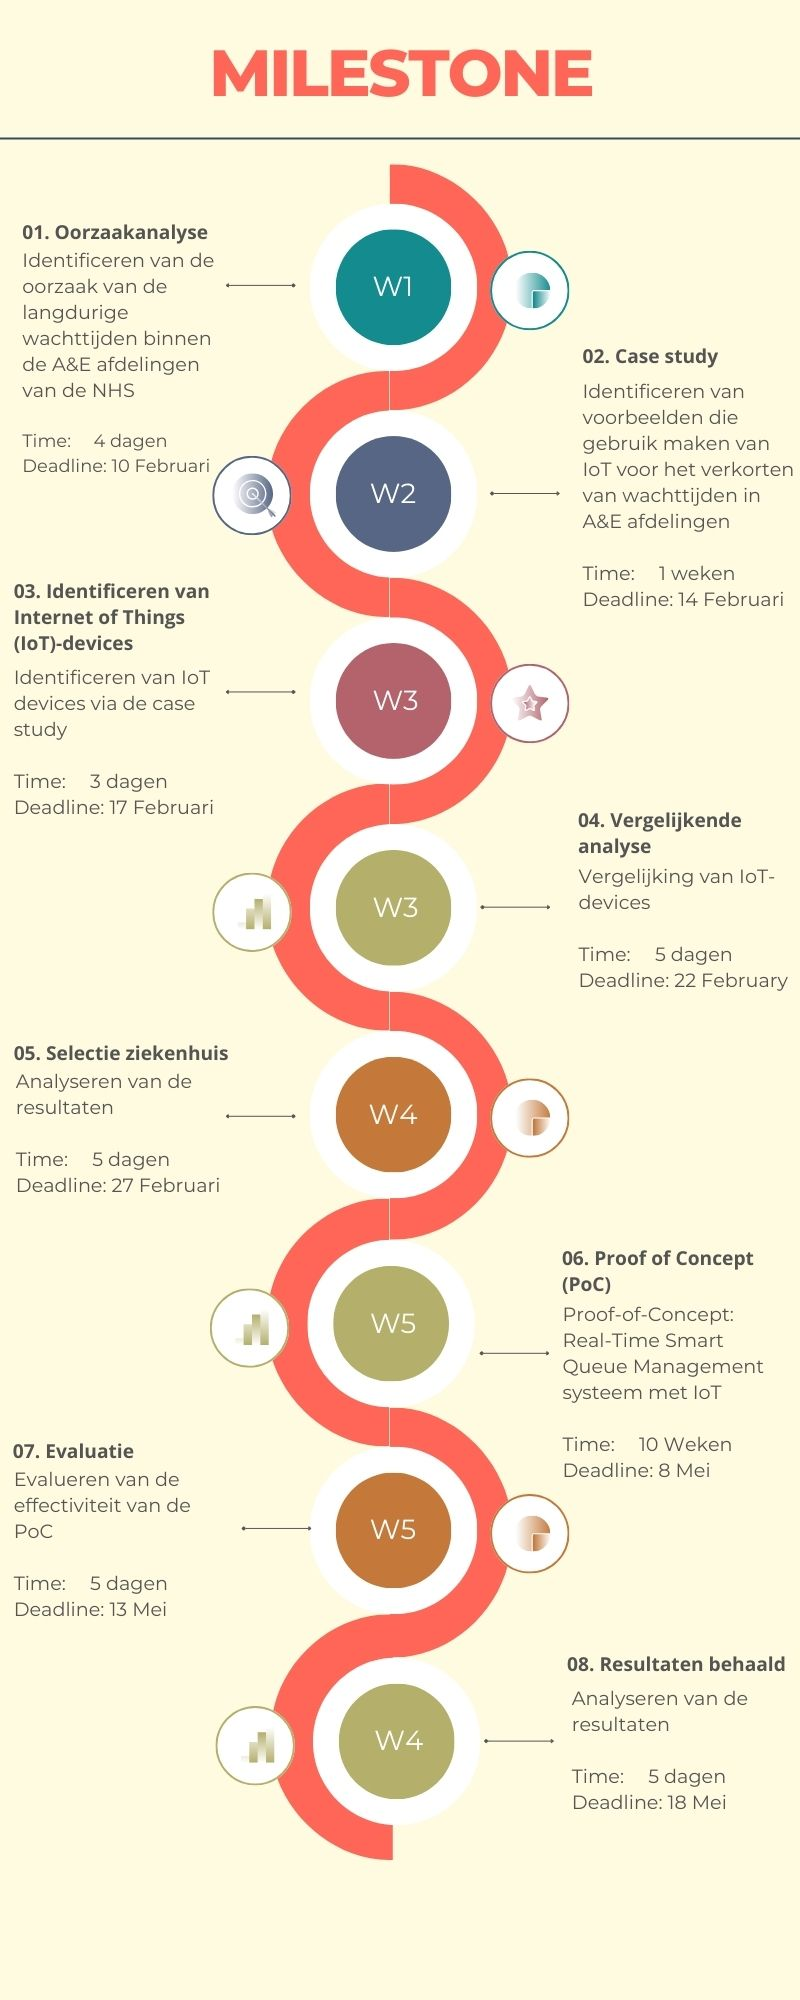
\includegraphics[width=0.92\linewidth]{img/milestone-4.png}
%    \label{fig:Figuur8}
%\end{figure}



%---------- Verwachte resultaten ----------------------------------------------
\section{Verwacht resultaat, conclusie}%
\label{sec:verwachte_resultaten}

% Hier beschrijf je welke resultaten je verwacht. Als je metingen en simulaties uitvoert, kan je hier al mock-ups maken van de grafieken samen met de verwachte conclusies. Benoem zeker al je assen en de onderdelen van de grafiek die je gaat gebruiken. Dit zorgt ervoor dat je concreet weet welk soort data je moet verzamelen en hoe je die moet meten.

% Wat heeft de doelgroep van je onderzoek aan het resultaat? Op welke manier zorgt jouw bachelorproef voor een meerwaarde?

% Hier beschrijf je wat je verwacht uit je onderzoek, met de motivatie waarom. Het is \textbf{niet} erg indien uit je onderzoek andere resultaten en conclusies vloeien dan dat je hier beschrijft: het is dan juist interessant om te onderzoeken waarom jouw hypothesen niet overeenkomen met de resultaten.


De verwachte resultaten van dit onderzoek zijn dat de proof-of-concept aantoont of het technisch haalbaar is om met IoT-sensoren betrouwbare bezettingsdata te verzamelen. Op basis van deze gegevens kan via Little’s Law en eenvoudige voorspellingsmodellen een inschatting gemaakt worden van de gemiddelde wachttijd. De studie beoogt niet om tijdens de meetperiode effectief een daling van de wachttijd te realiseren. In plaats daarvan ligt de focus op het opzetten van een meet- en voorspellingssysteem dat op termijn als onderbouw kan dienen voor optimalisaties van de patiëntdoorstroming. Indien de proof-of-concept stabiele en interpreteerbare data oplevert, kan dit als meerwaarde worden beschouwd voor ziekenhuizen die de inzet van IoT bij wachtrijbeheer overwegen.
